\section{Background and related works}
\label{sec:background}
\subsection{Multipath QUIC}
\label{subsec:MPQUIC}
% Le & Trung's text
%QUIC is a secure general-purpose transport protocol proposed by Google and standardized by IETF~\cite{rfc9000}. QUIC integrates TLS handshake, and the purpose is to allow an exchange of application data as soon as possible. Additionally, an advantage of employing this protocol is the prevention of head-of-line (HoL) blocking among various streams. In the event of a lost packet, only the stream that has data loss is blocked, as they must wait for data retransmission to arrive. Meanwhile, the remaining streams still continue without being affected. The outstanding advantages of QUIC, along with the successful implementation of Multipath TCP (MPTCP), have promoted the deployment of Multipath QUIC~\cite{mpquic}. Similar to MPTCP, MPQUIC can utilize multiple interfaces simultaneously (e.g., WLAN and LTE/5G) on a device, enhancing the robustness and performance of QUIC. MPQUIC achieves this by effectively combining multiplexing application streams and UDP subflows to leverage the advantages of multiple accessible networks~\cite{mpquic2}. 
% The network stacks of TCP/TLS, MPTCP, QUIC, and MPQUIC are compared in~\figref{fig:mpquicarc}. 

% Kien slightly modified
QUIC is a secure transport protocol, proposed by Google and standardized by IETF~\cite{rfc9000}. QUIC integrates TLS handshake, and the purpose is to allow an exchange of application data as soon as possible. Additionally, QUIC can prevent head-of-line (HoL) blocking among various streams. When a lost packet happens, only the affected stream is blocked, as it must wait for data retransmission to arrive. Meanwhile, the remaining streams continue without being affected. The advantages of QUIC, along with the successful implementation of MPTCP, have promoted the deployment of MPQUIC~\cite{mpquic, 8422951}. Like MPTCP, MPQUIC can simultaneously utilize multiple interfaces (e.g., WLAN and LTE/5G) on a device, enhancing robustness and performance. MPQUIC achieves this by effectively combining multiplexing application streams and UDP subflows to leverage the advantages of accessible networks~\cite{mpquic2}. 

% \begin{figure}[t]
% \centering
% 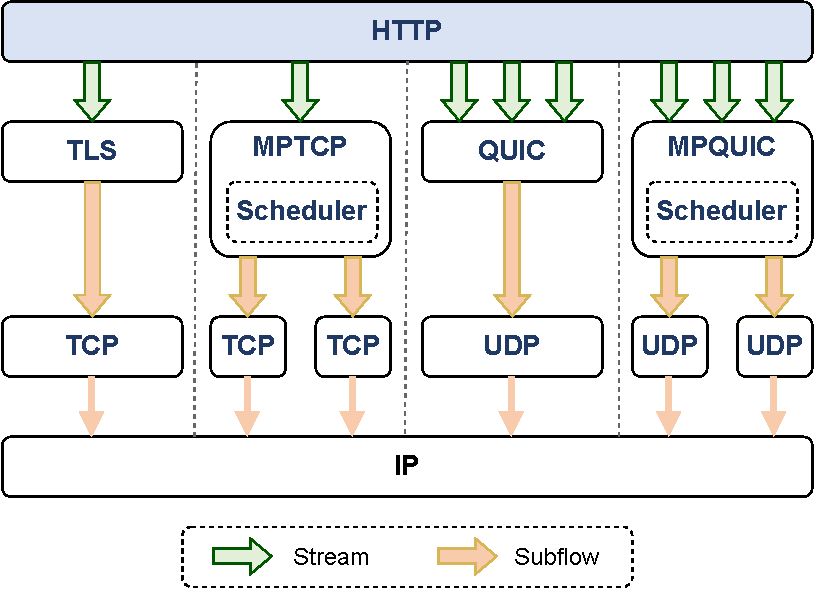
\includegraphics[width=8.5cm]{figs/ccnc-mpquic.pdf}
% \caption{Network stack of TCP/TLS, MPTCP, QUIC, and MPQUIC} \label{fig:mpquicarc}
% %\vspace{-0.1cm}
% \end{figure}
% \begin{figure}[t]
% \centering
% 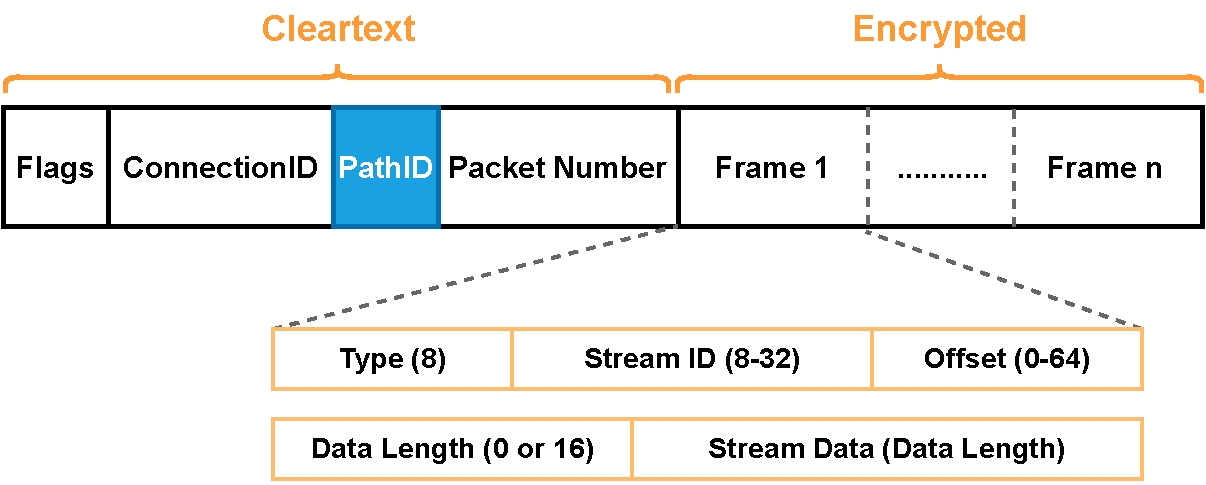
\includegraphics[width=8cm]{figs/ccnc-mpquicpacket.pdf}
% \caption{The format of a MPQUIC packet} \label{fig:mpquicpacket}
% %\vspace{-0.5cm}
% \end{figure}

\subsection{Existing MPQUIC schedulers }
\label{subsec:schedulers}

% Kien slightly modified
MPQUIC's default scheduler, minRTT~\cite{mpquic}, selects the path with the lower RTT and available CWND to transmit packets. When this path is unavailable, it continues to select the path with the lowest RTT in the remaining available paths. As a result, a challenge faced by minRTT is ignoring the possibility that the overall transmission time can be better by waiting for the lower-RTT path to become available again. BLEST~\cite{blest} and ECF~\cite{ecf} address the limitation and introduce a waiting mechanism to balance high throughput and low latency.

Under normal circumstances, when all paths have sufficient CWND, BLEST behaves similarly to minRTT. However, if the lower-RTT path is currently unavailable, BLEST evaluates whether to transmit data on a higher-RTT path or wait until the lower-RTT path becomes available again. Furthermore, BLEST considers the potential for HoL blocking during the transmission of large data volumes and makes decisions to minimize such risks. Similarly, ECF also employs a waiting mechanism similar to BLEST, but it calculates the benefit of reducing idle time on the path with the lower RTT. Additionally, ECF examines the packet arrival time for each path before scheduling, thus reducing the number of out-of-order packets. Despite the advances made by BLEST and ECF, the dynamic nature of wireless networks (e.g., significant latency variations), can diminish the performance of scheduling algorithms based on predefined policies~\cite{10152217}.

To address the challenges of network dynamicity, a learning-based approach called Peekaboo~\cite{peekaboo} is recently introduced. Peekaboo is still primarily based on minRTT, but employs a reinforcement learning-based decision-making technique when the lower RTT path is unavailable. Peekaboo operates in two phases: the learning phase and the deployment phase. In the learning phase, the multi-armed bandit model is used to learn optimal path selection from feature collection, including CWND, Send Window (SWND), Bytes in flight (BiF), and RTT. Subsequently, Peekaboo schedules packets over multiple paths using the learned policy during the deployment phase. Moreover, Peekaboo periodically evaluates the learning state in this phase and returns to the learning phase if a predefined threshold is reached. However, Peekaboo has some drawbacks. First, it relies on a fixed threshold to trigger the learning phase, limiting its adaptability to network dynamicity. Second, Peekaboo's decision-making is still based on minRTT, resulting in its performance converging with the performance of other minRTT-based schedulers as the available paths become more homogeneous in terms of RTT~\cite{10060683, mpeekaboo}.

\subsection{Q-learning}
\label{subsec:Q-learning}
Reinforcement learning encompasses various algorithms, with Q-learning standing as one of the most prominent and widely used methods~\cite{watkins1992q}. The fundamental concept behind Q-learning involves evaluating the desirability of state-action pairs using state-action values and iteratively updating these values over time. To accomplish this, Q-learning relies on a Q-table, effectively mapping the state-action space $\mathcal{S}$ and $\mathcal{A}$ to a numerical space $f:\mathcal{S} \times \mathcal{A} \to \mathbb{R}$. Upon convergence of state-action values, the agent's decision-making process is guided by a value-based policy. The core of Q-learning is a Bellman equation, which is used to update the Q value: 
\begin{equation}
\label{eq:bellman}
\small
\centering
Q_{(s^t, a^t)}^{new} \leftarrow (1-\alpha)Q_{(s^t, a^t)} + \alpha \left[R^{t+1} + \gamma \max_{a^{t+1}} Q_{(s^{t+1}, a^{t+1})}\right],
\end{equation}
where $(s^t, a^t)$, $(s^{t+1}, a^{t+1})$ represent current and next state-action pair, respectively. $R^{t+1}$ denotes the reward which is received by the agent at time step $t+1$. The learning rate $\alpha$ and discount factor $\gamma$ are scalar values within the range of $(0,1)$, determining the algorithm's learning speed and future reward importance, respectively. At each time point, the agent takes an action $a^t \in \mathcal{A}(s^t)$, observes the reward signal $R^{t+1}$, and transitions to the new state $s^{t+1}$. Subsequently, the agent updates the corresponding Q-value in the Q-table using the computed values.

